\documentclass[11pt]{article}
\usepackage{a4, fullpage}
\usepackage{bibtopic}
\usepackage[small,compact]{titlesec}
\usepackage{float}
\usepackage{amssymb,amsmath}
\usepackage[T1]{fontenc}
\usepackage{graphicx}
%\usepackage{multicol}
%\usepackage{multirow}
%\usepackage{listings}
%\usepackage{pdfpages}
%\usepackage{booktabs}

%\restylefloat{table}

%\setlength{\parskip}{0.3cm}
%\setlength{\parindent}{0cm}
%\setlength{\textheight}{10.7in} %used to be 10
%\setlength{\textwidth}{6.5in}
%\setlength{\parskip}{2pt}
%\addtolength{\oddsidemargin}{-.3in}
%\addtolength{\evensidemargin}{-.3in}
%\addtolength{\topmargin}{-.6in}
%\addtolength{\textwidth}{.6in}


\begin{document}

%-------------------------------------------------------------------------------

%\title{\vspace{100px} BUSINESS PLAN \\ \vspace{100px} Shimla Gold Cider \vspace{100px}}
%\author{\vspace{50px}John Walker, Rutwik Shah, Sahil Jain, Alina Boghiu, Giovanni Charles, Łukasz Koprowski \vspace{50px}}

%Imperial College London, Department of Computing

%\date{\today}         % inserts today's date

%\maketitle           % generates the title from the data above

%\newpage

%\title{ \hspace{100px} SHIMLA GOLD CIDER BUSINESS PLAN}
%\maketitle

%\begin{table}[H]
%\begin{center}
%\begin{tabular}{| l | l |}
%\hline
%Date Stamp of this Document:     &  \today  \\ \hline
%Version of this Document:        &  V.0.2   \\ \hline
%Author/Editor of this Document:  & Adam Fiksen, \newline Alina Boghiu, \newline Giovanni Charles, \newline John Walker, \newline Rutwik %Shah, \newline Sahil Jain, \newline Lukaz Koprowski  \\
%\hline
%\end{tabular}
%\end{center}
%\end{table}


%-------------------------------------------------------------------------------

%-------------------------------------------------------------------------------
%    ALTERNATIVE TITLE PAGE
%-------------------------------------------------------------------------------

\begin{titlepage}
\newcommand{\HRule}{\rule{\linewidth}{0.5mm}}
\center
\textsc{\LARGE Imperial College London}  \\[1.5cm]
\textsc{\Large Department of Computing}  \\[0.5cm]
\textsc{\large Course 350: Management and Business for Computing Engineers} \\[0.5cm]

\HRule \\[0.3cm]
{\huge \bfseries Business Plan \\ \vspace{0.3cm}Shimla Gold Cider} \\[0.3cm]
\HRule \\[1.5cm]
\begin{minipage}{0.4\textwidth}

% author
\begin{flushleft} \large \emph{Authors:} \\
Alina     \textsc{Boghiu}    \\
Giovanni  \textsc{Charles}   \\
Adam      \textsc{Fiksen}    \\
Sahil     \textsc{Jain}      \\
\L ukasz  \textsc{Koprowski} \\
Rutwik    \textsc{Shah}      \\
John      \textsc{Walker}    \\
\end{flushleft}

% supervisors
\end{minipage}~
\begin{minipage}{0.4\textwidth}

\begin{flushright} \large \emph{Lecturer:} \\
Nick \textsc{Coutts}
\end{flushright}
\end{minipage}\\[4cm]

%
\includegraphics[width=\textwidth]{apples.jpg}
\end{titlepage}

%-------------------------------------------------------------------------------
\title{DISCLAIMER}
\maketitle

\noindent Although the authors has taken reasonable care to ensure that the information contained in this document is accurate, no other representation or warranty, express or implied, is or will be given by the authors or any of its agents.No responsibility is or will be accepted by the authors or any of its agents as to the accuracy or completeness of this document or the information or opinions contained herein.Recipients must make their own investigations and must satisfy themselves as to the condition and prospects of the authors and the accuracy and completeness of statements contained herein. \\

\noindent This business plan has been prepared by the authors and is being provided to a limited number of persons, at their request. This document is confidential and is only being made available to parties who agree to keep it confidential. Neither this business plan nor any part of it shall be copied, reproduced or distributed to others at any time without the prior written consent of the authors. By accepting this document the recipient is deemed to undertake and warrant to the authors that the recipient will keep it confidential and that the recipient shall return all copies of this document to the authors immediately upon request. \\

\noindent Any financial projections given in this plan are illustrative only. Because of the early stage nature of the authors’ business, none of the projections given in this document should be taken as guaranteed to be attainable, nor should they be taken as implying any indication, assurance or guarantee that those assumptions are correct or exhaustive.
\vfill
\begin{table}[H]
\begin{center}
\begin{tabular}{| l l |}
\hline
Issued To:      &  Nick Coutts        \\
Company:        &  Shimla Gold Cider  \\
Date of Issue:  &  \today            \\
Copy Number:    &  1                  \\
\hline
\end{tabular}
\end{center}
\end{table}

\newpage
\tableofcontents

\newpage
%------------------------EXECUTIVE SUMMARY-------------------------------------%
\section{Executive Summary}
  \subsection{Overview}

  %A patented solution...
  %Vision to be...
Our mission is to bring a mid priced cider to the people of India. India has the second largest population in the world, and has an estimated market size of 500 million alcohol consumers [better estimate]. At the moment, there is one provider of cider in India, and we would like the change that. \\

\noindent We want to be a brewery. We will brew our own cider in the state of Himachal Pradesh, which is the source of the majority of the apples in India. Along with producing cider, we will sponsor other exclusive bars and clubs. \\

\noindent Operating in India which is well known for its corruption, we want to practice ethical development. eg corrupt free, no bribes, no blood cider forced labour fairtrade \\

\noindent We hope to gain popularity in major establishments, in Delhi and Mumbai through the open minded youth and bar owners. \\

\noindent Our cider will become a desired commodity through exclusivity and we will be able to research our market further at this point with minimal risk. \\

\noindent We will adapt and pick up popularity and scale up to make it available to the public.
  %Consumer and regulatory pressure...
  %Has clear competitve advantages...
  %Has unsurpassed technology and has sales through...

  \subsection{Market Drivers}
Marketing is all about creating value for the customer and striving to meet and then exceed customer expectations.\\

\noindent Market driver or drivers are considered at the time envisaging and establishing value of a product/service that's to be marketed. \\

\noindent These drivers are primarily trends that cause an existing or new market to develop. In our case, There is a large market for alcohol in India, who are eager to try out new things, which can be seen by the successes of these microbreweries. As India continues to grow to become a bigger powerhouse in the world, it will attract more foreigners, which means that people who already know about cider and like it will increase in the country. This increasing market size makes us believe that cider will become increasingly popular in India once introduced properly. \\

\noindent The four elements of segmentation especially psychographic and behavioral segmentation are key tools in determining these trends. \\

\noindent So at the end of the day, you'll be able to then understand how and why the market is changing, causes of the change and eventually looking out the window that will show how new opportunities are developed. \\
  %Market drivers....

  \subsection{Business Proposition}
  %Meets increasing demands...

  \subsubsection{Timeline}
After marketing planning and researching the development process we have decided upon a 7 month timeline for our business plan, encapsulating everything from setting up to starting the distribution of our product. The latter constitutes the end point of our business plan and a stable milestone after which the company can be considered self sustainable. Following are the three main stages of our timeline.

  \begin{enumerate}
  \item Licencing and building - 1 month
    \begin{itemize}
    \item Registr company
    \item Obtain brewing licence
    \item Rent space
    \item Setup utilities: contracts and infrastructure
    \end{itemize}

  \item Staff recruitment - 1 month
    \begin{itemize}
    \item Advertise job availability
    \item Process applications and interview applicants
    \item Start the training process as soon as we hire a qualified individual (brew master)
    \item Order equipment: it should have time to arrive by the time training is finished
    \end{itemize}

  \item Market research - 5 months\\
  This phaze constitutes of daily iterations of the following sequence:
    \begin{itemize}
    \item Produce small quantities of a recipie variation (with an offset of 20 days for fermenting)
    \item The professional taster tests the product and offers feedback
    \item The team and brewmaster distribute to locals and collect feedback
    \item The team and brewmaster reach out to distributers with samples of the product we are perfecting
    \item File for a patent on our final recipe. 
    \end{itemize}
  \noindent After 5 months the recipie should be perfected and contracts with distributors signed. The only change that must be made at this point is upping the production scale to meet the request. The equipment will be in place for this.
  \end{enumerate}

  \subsection{Financial Summary and Investment Proposition}
     For our Initial investment we require at current conversion rate an initial amount of Rs. 11,00,000 due to the large number of us participating in this project we do believe this amount is small enough for us to raise this through friends and family. We do believe starting a small business through this will provide us with flexibility to create a business model without having to answer to anyone. If run correctly, it will give the us the opportunity to earn more, with more freedom and independence.\\
     The First 9 months we intend to set up our brewery and perfect our product. This also provides time to market our product and spread word of its release. After this we intend to release the product into a few major cities through distributors

\newpage
%------------------------------------------------------------------------------%
%------------------------MARKET OPPORTUNITY------------------------------------%
\section{Market Opportunity}
  \subsection{The Opportunity for Shimla Gold Cider}

India is an increasingly growing economy where the common man is getting richer by the day. As people are getting richer, they are getting more money to spend on pleasure. Due to this increase in flux of money, people are willing to pay more than they used to on going to bar/pubs, which has become a common night out for the population. \\

\noindent As the demand for alcohol increases, we have found an untapped market. Currently, there is only one manufacturer of cider in India, which itself is becoming increasingly popular. In 2006 in the United Kingdom, 600 million litres of cider are produced annually. Beer is very popular in India, and it has been growing steadily at a rate of 10\%-17\% over the past 10 years. Around 170 million cases (12 bottles) of beer were produced in the financial year 2008-2009. \\

\noindent These figures indicate that there can potentially be a large market for cider in India, and we believe that Shimla Gold Cider can make it big in India if it is produced and marketed well. \\

\noindent As we can see, there is a large market for alcohol in India, who are eager to try out new things, which can be seen by the successes of these microbreweries. As India continues to grow to become a bigger powerhouse in the world, it will attract more foreigners, which means that people who already know about cider and like it will increase in the country. This increasing market size makes us believe that cider will become increasingly popular in India once introduced properly.
  %Addressable market of... 
 
  \subsection{Market Segments}
  %Clear market segments Including...

\newpage
%------------------------------------------------------------------------------%
%------------------------PRODUCT PROPOSITION-----------------------------------%
\section{Shimla Gold Cider Product Proposition}
%Has superior technology in....
  \subsection{Shimla Gold Cider's Unique Proposition}
Our product is proven cost effective and easy to implement. We have researched a number of recipies and asked one person about their home brewing experience. They clearly explained the process of brewing cider, which is straight forward and reasonably fast such that selling the produce can easily cover production cost and return profit in early stages. \\

\noindent We are planning to operate as a microbrewery producing small volumes of cider. We will start by conducting experiments and testing various recipes to find one which will be most suitable for Indian market. This testing phase significantly reduces our production power as we have to be able to operate quickly and modify recipes according to feedback. \\

\noindent We need two types of specialists to operate effectively as microbrewery. These are two initial recipes for our ciders, which we use to estimate cost and quantities of raw ingredients that will be needed. They are most likely to change, and both quantity and exact ingredients will vary depending on the cider recipe development process and the decisions of the brewing master.

  \begin{enumerate}
    \item Ingredients for dry, sparkling cider, 10.5\% abv (per gallon of cider)
	  \begin{itemize}
	   \item Apples - 7kg
	   \item Yeast (English Cider) - 2g
	   \item Campden tablets - 1
       \end{itemize}
	\item Ingredients for sweet, sparkling cider,10.5\% abv (per gallon of cider)
	  \begin{itemize}
	  \item Apples - 7kg
	  \item Yeast (Sweet Mead) - 2g
	  \item Sugar - 250g
	  \item Campden tablets - 1
	  \end{itemize}
	\end{enumerate}

  \newpage
  \subsection{Business Model}
  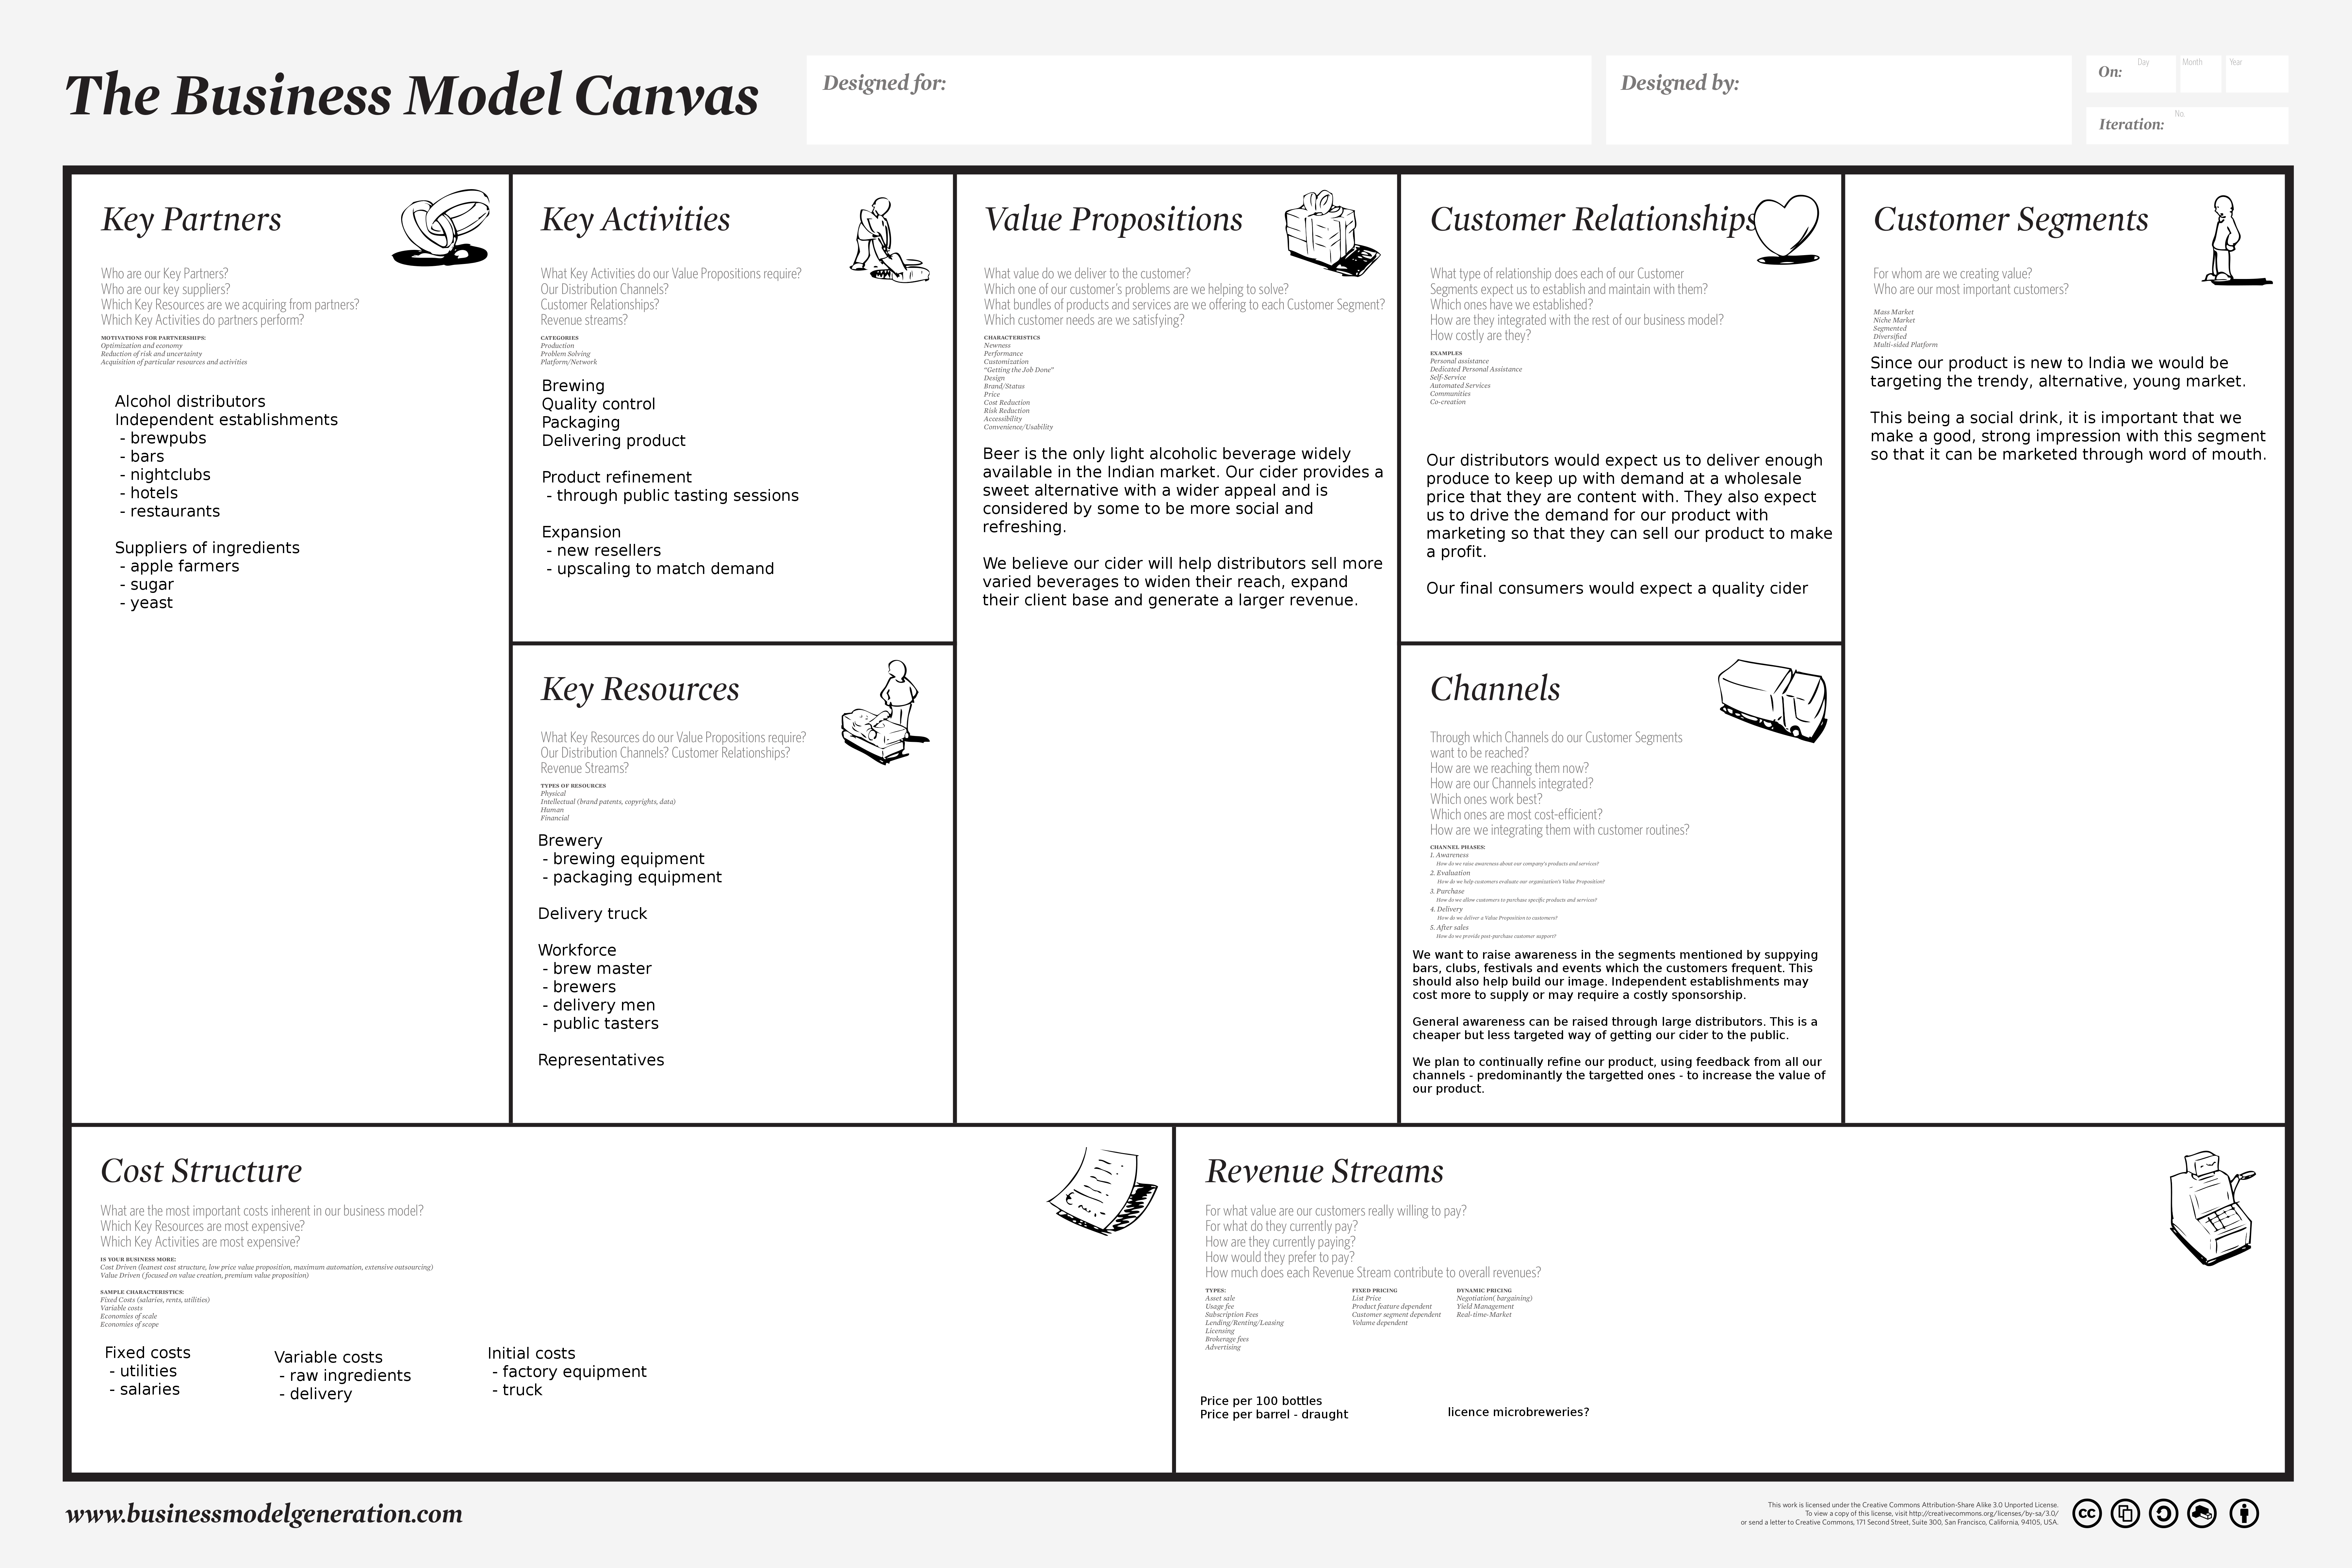
\includegraphics[angle=90,width=\textwidth,height=\textheight,keepaspectratio]{./business_model_canvas_poster.png}
   %Established production, sales & marketing, distibution model...

\newpage
%------------------------------------------------------------------------------%
%------------------------TARGET MARKET-----------------------------------------%
\section{Target Market}
  \subsection{Market Context}
  %Global vision well defined market segments and territories...
  \subsection{Market Size and Characteristics}
  %This equates to a global revenue opportunity of??? 
  %Diagram yearly market potential
  \subsection{Market Validation}
  %Has met all technical norms

\newpage
%------------------------------------------------------------------------------%
%------------------------COMPETITION-------------------------------------------%
\section{Competition}
%Limited number of direct competitors
	\subsection{Current Competitors}
There is only one manufacturer of cider in India at the moment. Green Valley Cider produces Tempest Cider, which is a 8\% cider, in the state of Himachal Pradesh, where they own several acres of apple orchards. Tempest cider are sold at Rs 60/- per 330ml bottles, and for Rs 105/- per quart. The most recent figures of Tempest Cider sales indicate that in 2007, around 50,000 cases of 12 bottles each were being sold annually. Currently, Tempest Cider is not available in the big cities of India such as New Delhi and Mumbai. \\

\noindent Some exclusive alcohol stores in India sell imported ciders, but these are very rare. The price of these imported ciders is very high as well, due to the high 150\% alcohol import tax.

  \subsection{Competitive Advantage}
  %Competitve advantage in technology

\newpage
%------------------------------------------------------------------------------%
%------------------------MARKET DEVELOPMENT PLAN-------------------------------%
\section{Market Development Plan}
  \subsection{Sales Process}
  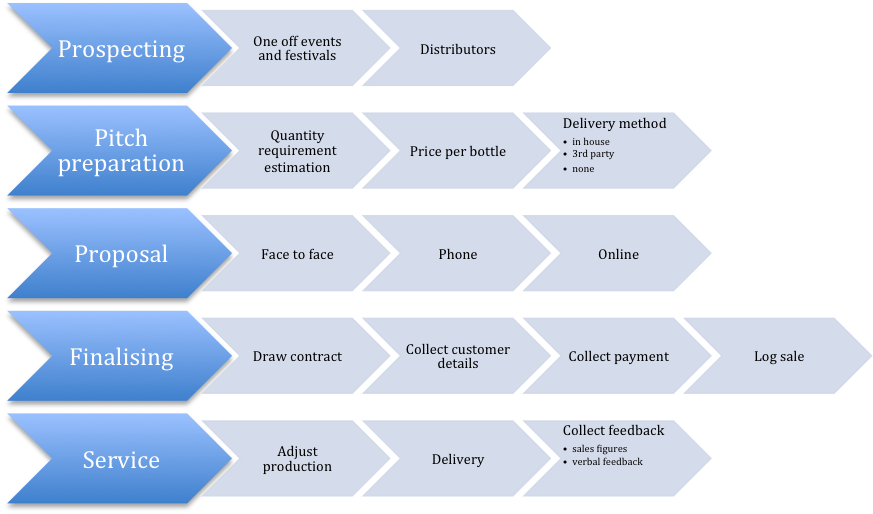
\includegraphics[width=\textwidth,keepaspectratio]{./process.png}
  %Good relationship with strong distributor...

  \subsection{Target Customers}
  %Larger customers as targets

  \subsection{Current Key Customers}
  %Large current customers

  \subsection{Marketing, PR and Communications}
  %Marketing and market awareness crucial..
We aim at advertising at horse racing events this has a cost of Rs. 5,00,000 though this number is high it has several benefits in doing so:
\begin{enumerate}
\item Conduct contests of skill and award prizes to the public to generate interest. 
\item Advertise on the CCTV transmission at all centers .
\item Have full rights for on-site branding across the stands.
\item Name the race to suit its preference.
\item Have its CEO / nominee present the trophy.
\item Be entitled to the free use of lawns above a certain value of sponsorship.
\item Arrange for live entertainment at race time or before or after the event.
\item Promote and your brand the race via mailers/press.
\item Have access to the Club's membership data which consists of thousands of potential customers who represent some of the most well off clients in India.
\item Have promotion on the website with links to the lounges webpage.
\item Get coverage on a major television network as these races will be viewed world wide.
\end{enumerate}

\newpage
%------------------------------------------------------------------------------%
%------------------------INTELLECTUAL PROPERTY (IP) ASSETS---------------------%
\section{Intellectual Property (IP) Assets}
  \subsection{Shimla Gold Cider Solution}
    \subsubsection{Patents}
    Cider is an age old product and we are using already existing machinery to 
    produce it therefore the number of patents we can take out is limited we will
    be looking to take out the following patents.
    \begin{itemize}
    	\item Recipe \\ 
We will be looking to take out a patent on the recipe for our cider this means the recipe has to meet 4 criteria:
 	      \begin{itemize}
		  \item It has to be patentable subject matter, a recipe is a new 'composition of matter' therefore it is patentable.
		  \item It has to be useful. Virtually everything is considered useful.
		  \item Is it novel and non-obvious. This might be harder to prove as cider is such an age old recipe but we could argue that our new use of Indian Shimla apples is novel
	      \end{itemize}
If we fail to obtain a patent on our recipe we would have to resort to simply keeping the recipe a secret this has worked for many companies in the past. Our recipe will be a unique blend of various types of apple and flavour brewed in a particular way using particular equipment it will be very hard to reproduce and by the time any one had we would hopefully have a large market share making it harder for competitors. 
	\item Name \\
    We will be looking to trademark the name of Shimla Gold Cider.
	\item Logo \\
    We will also be looking to patent the logo for Shimla Gold Cider.
    \end{itemize}
Obtaining these patents will cost around £220.\textbf{[this belongs in the finaince secion]}

    \subsubsection{Know-How}
    %Internation experts choose to work with X

  \subsection{Future IP Developments}
  %Future applications plannes along with IP Protection...
Although not as pressing as our cider, we will also be looking to to take of patents soon after we start production of the the cider for our subsidiary apple juice product this will include the recipe, name and logo. Obtaining these patents will cost a further £220. \textbf{[this belongs in the finaince secion]}

\newpage
%------------------------------------------------------------------------------%
%------------------------BUSINESS GROWTH AND RESOURCE PLANS--------------------%
\section{Business Growth and Resource Plans}
In order to setup a stable and longlasting infrastructure for our business we must take into consideration all the stages and requirements of production. Reaserching our cider recipe constituted the guideline and starting point of a coherent development plan. 

  \subsection{Current Structure and Resources}
  %Early phase centred on technology development
The favourable aspects of our current situation is our team of young, dynamic individuals, excited about implementig a good business idea. We are fast learners, on our way to obtaining university degrees, with a great tolerance to change and fully capabale of taking on unforseen obstacles without being overwhelmed by minor defeats. We believe a positive, persistent and energetic attitude towards implementig any business will yield a positive result and a great learning experience.

  \subsection{Straff Recruitment}
%The average cost of hiring for the skilled workers is about 1,00,000 a year we would require :
% Keep all the cost and finance information in one well defined section
  \begin{enumerate}
  \item Qualified Brewmaster \\
He has to have previous experience with brewing various types of cider and would probably have to be recruited from a country with cider making traditions (France, England). He would serve as our cider making expert, being able to swiftly operate the equipment and professionally asses the quality of our cider. He must also supervise the general staff activity and behaviour.

  \item Microbiologist \\
He would serve as an assistant brewmaster, and would be responsible for conducting cider quality control tests, and performing microbiological analysis. He must also verify all the ingredients including the apples, sugar, yeast and water.
It is important to ensure a good quality especially considering the novelty of our product for this market.

  \item Unqualified labour \\
Our microbrewary requires manual labour as described below. These employees must work with the equipment we provide, attend to washing and maintaing it with resposability. Therefore brief training must be considered as a cost. \\ 
  2 workers in charge of apple receival, washing and sorting
  2 workers in charge of apple grating
  2 workers in charge of apple pressing
  1 worker in charge of general cleaning of the area

  \item Security guard \\
On top of general surveillence, he is in charge of verifying employee ids and greeting visitors.
  \end{enumerate}

% same here, all cost information in one place
% Further as required we will require a security guard which will cost about Rs. 50,000 a year.
 
  \subsection{Facilities}
    \subsubsection{Space requirements}
When deciding upon our homebase we considered firstly our situation as a new business, with no existing assets or experience, as well as the small scale of our production line. \\

\noindent We are aiming to brew \emph{15 gallons per day}. Whilst we will start off by brewing small qunatities in order to perfect the recipe, we must setup the scale which we need for efficient and profitable distribution. We have already identified the ingredients qunatity requirements per gallon when researching the recipies we will use and have explained how these might change. Using this information, these are the room size and functionality requirements we identified: \\

  \begin{enumerate}
  \item Ingredients handling room \\
  This room must be easily accessible by our providers and large enough to store a week's worth of ingredients including:
    \begin{itemize}
    \item 1500L refrigerator to store 630Kg of apples
    \item 23kg of sugar
    \item yeast, campden tablets
    \end{itemize}
  The room must have a constant supply of water for washing apples and equipment. \\
  The room will operate a weekly pipeline of ingredients storage, however spare space must be available for unforseen situations.\\
  The room size must also allow washing, grating and pressing of apples which implies equipment and staff as detailed in the following sections.

  \item Brewing room \\
  This room must accomodate the two brewing systems for dry and sweet cider: aproximately $2m^3$ each. It must also be able to fit a desk and file cabinet for general office equipment.
  \item Fermenting room \\
  This room will operate a daily pipeline and must be able to accomodate a weeks worth of produce: $4m^3$. It must maintain a constant temperature of aproximately $22^\circ$C for fermentation. We have decided upon this as a good trade-off between quality and speed which are inveresely proportional: a lower fermenting temperature yelds higher quality but requires more time. However this is a specific decision the brewing master must make daily.

  \item Bottling and storage room \\
  The bottling room must accomodate enough space to hold our 2 kegs/day as well as the bottles the cider goes into -- assuming we produce about 20 gallons a day in full production, that requires about 230 bottles a day. The space required for this is roughly $1m^3$. We then need to take into account how regularly we will receive pickups from distributors --about one week. This results in a room of at least $7m^3$ for storage, plus space to actually perform the bottling. \\
The bottling work will be done with the use of `bottling wands' which allow a consistent amount of cider to be poured per bottle, as well as keeping the cider from oxygenating. For our fizzy ciders, we will introduce about 3.3g of sugar per bottle to allow secondary fermentation to occur. These filled bottles are then handed off to a capper, who will place the caps on each bottle, use the bottle capper to tighten the caps and place them in to boxes for storage.

  \item Maintainance room\\
  This should be a small room for storing cleaning equipment. It should have access or be attached to a staff restroom.
  \end{enumerate}

    \subsubsection{Equipment requirements}
    \begin{enumerate}
    \item Production equipment
      \begin{itemize}
      \item Apple wash tub
      \item Apple crushing device
      \item Hand cracked cider press: small
      \item Mash tank: 15 gallon
      \item Sparge tank: 15 gallon
      \item Boil Kettle with a false bottom and a siphoning tube
      \item Chill wizzard with a cold water hoze and oxigen pump
      \item Fermenting tank with blow up valves for speedup: 15 gallon
      \item Propane burner
      \end{itemize}

    \item Storage equipment
      \begin{itemize}
      \item 1500L refridgerator for apple storage
      \item freezer for excess and spare apple woat
      \item Fermenting tanks: as mentioned above, in order to host the weekly pipeline, we require 7 15 gallon tanks and spares.
      \item bottles: we are aiming for a production line of 210 bottles daily therefore our weekly requirements is of aproximately 1300 bottles including spares
      \item boxes and lables
      \item shelves or containers ingredients (which come in their own boxes)
      \end{itemize}

    \item General maintainance equipment
      \begin{itemize}
      \item airconditioning system: for the fermentation process
      \item security alarm ans surveillence system
      \item fire detection system
      \item water filtering system
      \item cleaning equipment:
        \begin{itemize}
        \item chemical substances (pbw socution, idophor)
        \item cleaning substances (soap, bleach)
        \item blue roll, toilet roll, cloths
        \item bags, bin bags
        \item hozes, gloves, brooms, mops, buckets
        \end{itemize}
      \item office equipment:
        \begin{itemize}
        \item paper and pens
        \item company stamp, files, plastic sleeves, paper punch, envelopes, stapler and spaples, disposable cups, bin
        \item employee register book, visitor register book
        \item company landline telephone
        \item company laptop
        \item tea, coffee, water
        \item first aid kit
        \end{itemize}
      \end{itemize}
    \end{enumerate}
\newpage
%------------------------------------------------------------------------------%
%------------------------FINANCIAL PLAN AND FUNDING ASSUMPTIONS----------------%
\section{Financial Plan and Funding Assumptions}
  \subsection{Financial History}
  \subsection{Financial Projections}
Initially our main source of revenue would stem from sale of products in the short run once we aim at establishing our brand through adverstising and selling through pubs. Gradually we would like to further increase volume of sales and production and increase revenue through sponsors. In the long run we would like to further increase our product range including different flavours of ciders and gradually streamline our distribution process. This will all result in economies of scale hence reducing cost and added prodict range will increase volume of sales.

\begin{center}
\begin{tabular}[width=\textwidth]{| c | c | c | c | c | c | c |}
\hline
Facilities and Equipment & Salaries and Rent  & Maintenence & Misc. & Raw Materials & Bills & Bonuses \\ \hline \hline
1000000                  & 375000             & 5000        & 10000 & 12500         & 15000 & 0       \\
5000                     & 375000             & 50000       & 10000 & 15000         & 15000 & 10000   \\
5000                     & 375000             & 50000       & 10000 & 17500         & 15000 & 12500   \\
5000                     & 375000             & 50000       & 10000 & 20000         & 15000 & 15000   \\ \hline
\end{tabular}
\end{center}

\begin{center}
\begin{tabular}{| c | }
\hline
Revenue \\ \hline
540000 \\
620000 \\
750000 \\
900000 \\ \hline
\end{tabular}
\end{center}

  \subsection{Use of Funds}
    \subsubsection{Staff Hiring and Property}
Since we aim at setting up a microbrewery to start with in at a manufacturing area in Himachal Pradesh

Rent in this area is roughly about Rs.1 / ft$^2$ per month.
As seen in the requirements:

there is a storage area required this has been estimated to: 500 sq $^2$ area of for manufacturing the product would be 1500 ft$^2$ this is plenty to space to meet estimated current requirements

Lunch area and office space is estimated to be about 1000 $^2$ as well this as above well allows some space for hiring a few more employees if and when needed.

Hence yearly rent works out at Rs. 24,000 per year.
    \subsubsection{Ingredients}
cost of sugar -  Rs.30 / kg
campden tables  - Rs.300 per 100 tablets
Sweet mead Rs.500 for /128 gms 


This brings the cost of dry cider to Rs. 5.866 per 330 ml
This brings the sweet of dry cider to Rs. 6.4 per 330 ml

     \subsubsection{Equipment and Facilities}
     %Funds needed for sales and marketing support

\newpage
%------------------------------------------------------------------------------%
%------------------------EXIT STRATEGY-----------------------------------------%
\section{Exit Strategy}
%Exit-trade sale

\newpage
%------------------------------------------------------------------------------%
%------------------------RISK ANALYSIS-----------------------------------------%
\section{Risk Analysis}

  \subsection{Risk Assessment and Management}
Identyfying risks is mainly aimed at helping to outline a realistic budget requirement. Most of the items below are not avoidable, like staff illness or natural hazzards. However some are, and foreseeing even the unavoidable ones can make them more managable. Following is a comprehensive list of risks, including our approach to dealing with them.
   %Strong distribution channels minimise risk as does IP protection

  \begin{enumerate}
  \item Human related risks
    \begin{itemize}
    \item Delaied production \\ Wheather it is because of suppliers delivering ingredients late or to do with the quality of the delivered product, we should have either a week's worth safety batch, which implies buying a freezer, or be prepared to deal with the cost of delaied production.
    \item Late distribution \\
The small scale of our buiness means space is limited which may cause a problem if buyers are late with picking up the merchandise. We should consider having an emergenci courier  or again be prepared to deal with the const of delaied production.
    \item Experience of employees \\
Providing a training session is sometimes insufficient for ensuring perfect performance from our employees. We must be prepared to deal with the cost of flawed batches.
    \item Injuries, illness, misbehaviour \\
Anything that leads to an employee not being able to perform his tasks on a given day should be considered as a potential delay and extra cost. 
    \end{itemize}

  \item Equipment related risks
    \begin{itemize}
    \item Break down \\
The extra cost that comes with machines breaking down can be reduced by a good warantee on each piece of equipment, insurance and availability of spare parts.
    \item Power cut \\
Whilst inevitable, this risk can be couterbalanced if our contract with unilities providers includes compensations for this type of situation. We must also ensure our production can endure a long standby time and again be able to handle the cost of potentially loosing a batch.
    \item Water contamination \\
%not sure about this
The scale of our business does not permit a water filtering system which means we must test the quality of the provided water daily.
    \end{itemize}

  \item Ethical risks
    \begin{itemize}
    \item Working environment
    \item Religious employees
    \item Waste disposal \\
Waste disposal can be a sensitive issue with locals. Some of our waste may be have particularly unpleasant odor due to its biodegradable nature. We must try and find a way of donating apple residue to nearby farmers.
    \end{itemize}
  \end{enumerate}

\newpage
%------------------------------------------------------------------------------%
%------------------------COMPANY STRUCTURE AND MANAGEMENT PROFILES-------------%
\section{Company Structure and Management Profiles}
  \subsection{Current Equity Structure}
  %Clear ownership structure
  \subsection{Management Team}
  %Expirences management team
  \subsection{Corporate Information}
  %Directors
  %Registered Number
  %Registered Office
  %VAT Number
  %Company Auditors
  %Company Lawyers
  %Company Bankers
  \begin{table}[H]
  \begin{center}
  \begin{tabular}{| p{7cm} | p{7cm} |}
  \hline
  Directors:  & Adam Fiksen, \newline Alina Boghiu, \newline Giovanni Charles, \newline John Walker, \newline Rutwik Shah, \newline Sahil Jain, \newline Lukaz Koprowski  \\
  \hline
  Registered Number & BLANK \\
  \hline 
  Registered Office & BLANK \\
  \hline
  VAT Number        & BLANK \\
  \hline
  Company Auditors  & BLANK \\
  \hline
  Company Lawyers   & BLANK \\
  \hline
  Company Bankers   & BLANK \\
  \hline
  \end{tabular}
  \end{center}
  \end{table}

  \subsection{Location and Contact Details}

\newpage
%------------------------------------------------------------------------------%
%------------------------ANNEX 1-----------------------------------------------%

\section{ANNEX 1 \\ Market Players}


\newpage

%------------------------------------------------------------------------------%
%------------------------ANNEX 2-----------------------------------------------%

\section{ANNEX 2 \\ Conclusion}
As a conclusion to our business proposition we would like to outline a few learning outcomes this experience has provided us with.\\

\noindent Fisrtly, being put in the situation of having to think about the implementation details of a business has shown us the benefits of being able to follow a well defined plan and the advantages of being organized as a team. Whilst the business idea might be fairly easy to explain, its implementation, however small the scale, raises an edless stream of problems to be solved and questiones to be answered which prove both the capacity and the limitations of human intuition. For this reason it is extreamly important to follow a rigurous plan and try to forsee as many risks as possible, as it is impossible to control the flow of events completely. \\

\noindent Secondly, we learnt there is much more to selling a product than making it available. Whilst a good product will advertise itself, tiit is important to sell the entire experience that goes with it and be prepared for both expantion or having to start over from scratch. Looking at success and failiure stories of other startups whilst trying to outline the plan for our own business developement, we saw that luck, whilst helpful, is replaceable with careful financial estimations, a pesimistic timeline and clever safety measures. \\

\noindent Finally, we saw that in order to make good use of resources and come accross as reliable the leading team must have well defined roles, in accordance with their skills. in order for potential investors to trust we can acomplish our goals, it is important to have a constant sense check when planning developement and remain realistic.\\

\noindent We consider this exercise to have been a worthwhile experience for having shown us a more comprehensive way of thinking about projects in general.

\newpage
%------------------------------------------------------------------------------%
%------------------------ANNEX 3-----------------------------------------------%

\section{ANNEX 3 \\ Company Background}
Shimla Gold Cider is the vision of 7 computing students from Imperial College London, we've all been good friends for a long time and last summer Giovanni and Adam went to visit Rutwik and Sahil in India, during their time there they made a peculiar observation that they couldn't find any cider in India. \\

\noindent They asked Sahil and Rutwik about this and they couldn't provide an explanation even in the areas of India frequented by cider accustomed westerners such as Goa, there was just no cider. At first we thought maybe the taste just didn't agree with the Indian culture but we know first hand that many of our Indian friends enjoy it when abroad, it just seemed that nobody had introduced it yet. \\

\noindent It was from this simple observation the idea to bring cider to the Indian market was conceived. Shimla is the area of India where apples were first introduced by Samuel Evan Stokes and remains the heart of apple cultivation today. Shimla was regarded and the capital of Summer time India by the British which we believe nicely reflects the Anglo-Indian dynamic of our team, we hope to add to the historic reputation of Shimla by making it the birth place of Shimla Gold Cider.

\newpage
%------------------------------------------------------------------------------%
%------------------------------------------------------------------------------%
\end{document}
